\section{Desugaring}
\label{sec:desugar}

%\begin{figure}[t]
%{\eightpoint
%\begin{verbatim}
%  int->int filter IterationFilter() {
%
%      work push 1 pop 1{
%
%          int counter = iter();
%          ...
%
%      }
%  }
%\end{verbatim}
%\caption{Example of a StreamIt filter using the iteration keyword.\protect\label{fig:iter-filter-example}}}
%\end{figure}
%
%
%\begin{figure}[t]
%{\eightpoint	
%\begin{verbatim}
%  int->int filter IterationFilter() {
%
%      int iter = 0;      
%
%      work push 1 pop 1{
%
%          int counter = iter;
%          ...
%
%          iter++;
%
%      }
%  }
%\end{verbatim}
%\caption{Example of a StreamIt filter with the iteration keyword desugared.\protect\label{fig:desugar-filter-example}}}
%\end{figure}


\begin{figure}[t!]
\centering
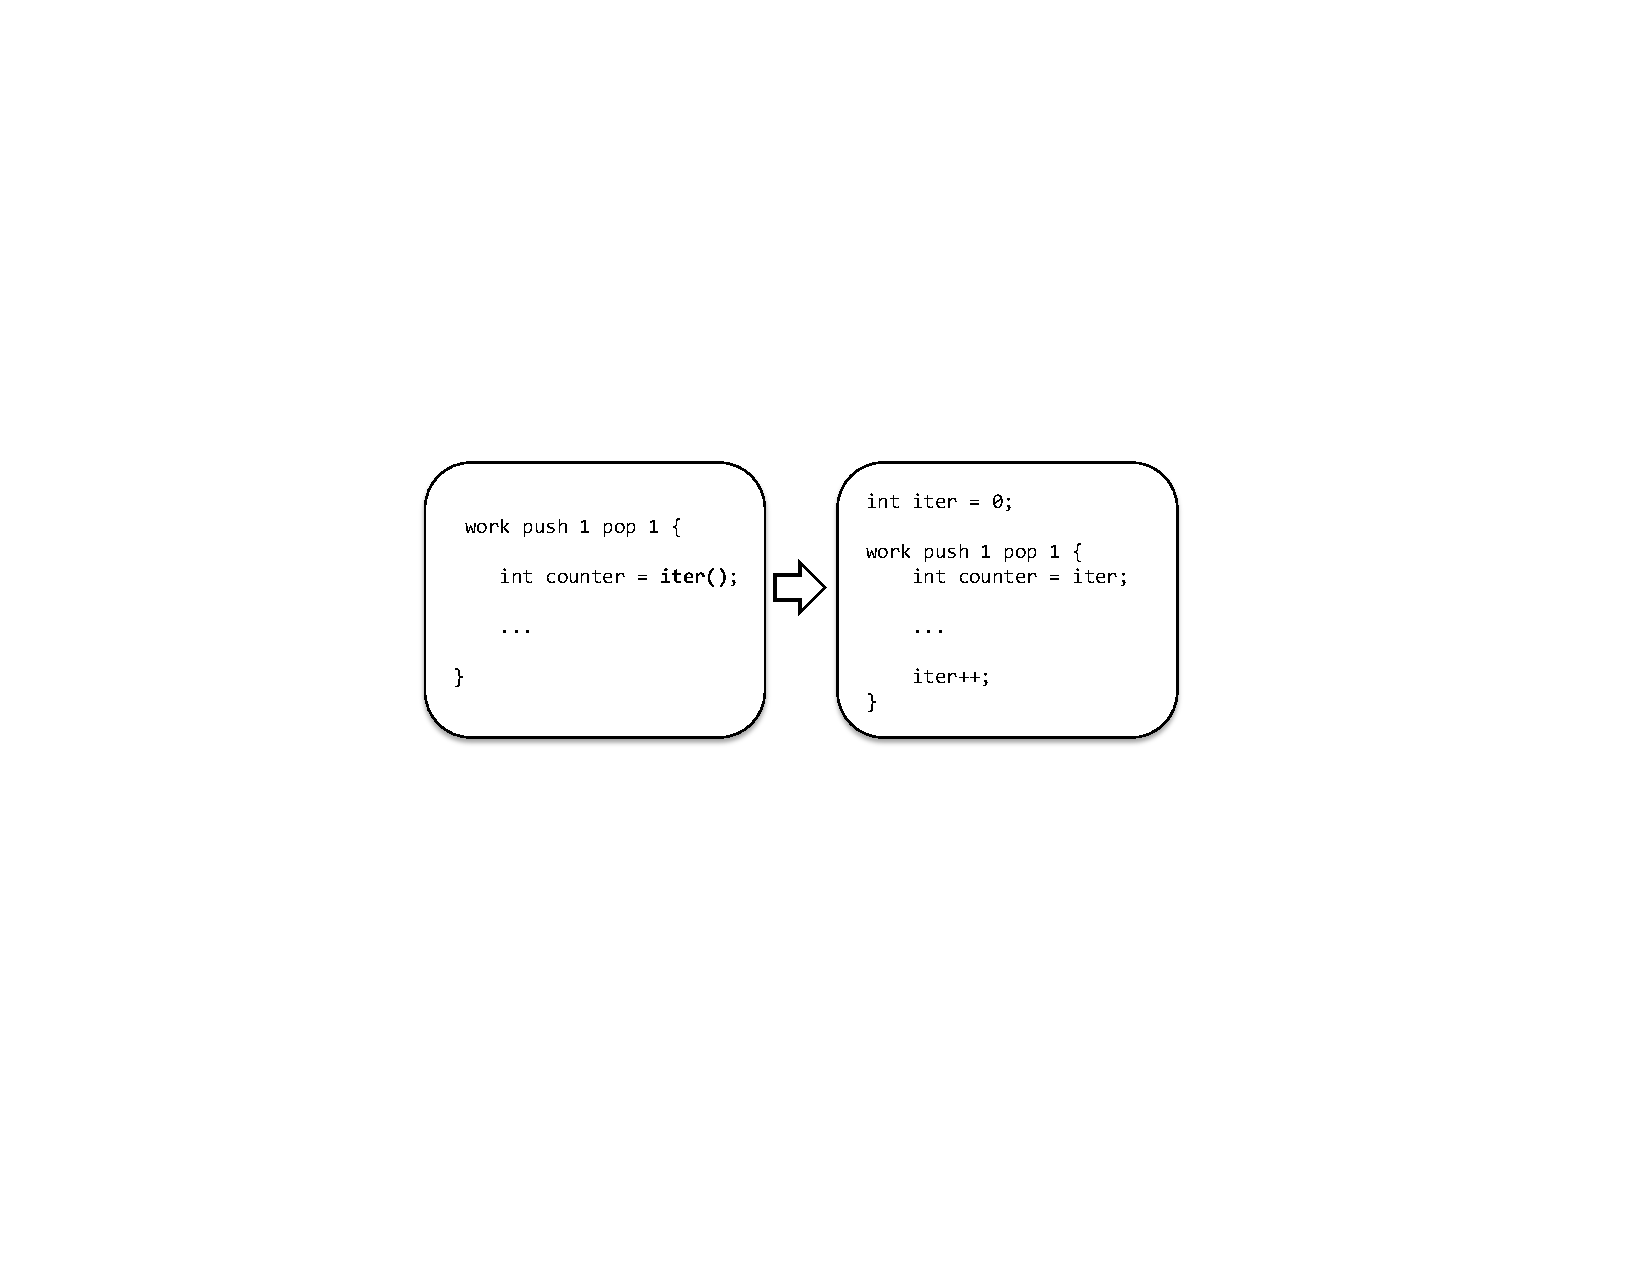
\includegraphics[width=3.3in]{figures/desugaring_filters.pdf} 
\caption{Desugaring a filter using \texttt{iter()} keyword.\protect\label{fig:desugar}}
\end{figure}


A filter is classified as an {\it iteration filter} when there exists a use of
\iter in its \prework or \work function.  In this section, we
introduce a simple desugaring transformation that will convert an
iteration filter into a filter that does not include the \iter
keyword, but implements the correct semantics of the \iter use.  We
accomplish this by introducing a state field that records the current
iteration of this filter.  This state field is updated in a consistent
and compiler-defined manner, so later transformations and passes (such
as fission, see \S\ref{sec:fission}) can reason about the
state.  

The \iter expression is replaced with an access to a field holding the
value of the iteration count.  Again, the filter is given a definition
of this field only if it is classified as an iteration filter, this
field is not added to non-iteration filters.  The \work and \prework
function (if it exists) are appended with incrementing statements that
update the iteration value.  The name of the state field is compiler
defined for easy recognition by later passes, for the remainder of
this paper the field is named {\it iter}.


Figure~\ref{fig:desugar} provides a code example of the desugaring
process.  The left filter in Figure~\ref{fig:desugar} shows an
iteration filter.  All references to the keyword are replaced to field
accesses to the {\it iter} field.  Figure~\ref{fig:desugar} shows the
StreamIt code representation after the iteration keyword is desugared.

% The introduction of this iteration field creates state in the provided
% filter.  For future operations, the compiler does not consider this
% iteration field as part of the state of filter.  Future processes will
% maintain this inherent state without the downsides of explicitly
% introduced state.

% It is important to note, these filters are not classified as stateful
% to the user, even though the filter is actually stateful on the
% iteration count after the desugaring process.  In classifying filters
% as stateful, the user is made aware of where data parallelism may be
% inhibited.  Iteration filters will not inhibit data parallelism
% because its state is identifiable to the compiler during the fission
% process.
